% Options for packages loaded elsewhere
\PassOptionsToPackage{unicode}{hyperref}
\PassOptionsToPackage{hyphens}{url}
\PassOptionsToPackage{dvipsnames,svgnames,x11names}{xcolor}
%
\documentclass[
]{article}
\author{}
\date{}

\usepackage{amsmath,amssymb}
\usepackage{lmodern}
\usepackage{iftex}
\ifPDFTeX
  \usepackage[T1]{fontenc}
  \usepackage[utf8]{inputenc}
  \usepackage{textcomp} % provide euro and other symbols
\else % if luatex or xetex
  \usepackage{unicode-math}
  \defaultfontfeatures{Scale=MatchLowercase}
  \defaultfontfeatures[\rmfamily]{Ligatures=TeX,Scale=1}
\fi
% Use upquote if available, for straight quotes in verbatim environments
\IfFileExists{upquote.sty}{\usepackage{upquote}}{}
\IfFileExists{microtype.sty}{% use microtype if available
  \usepackage[]{microtype}
  \UseMicrotypeSet[protrusion]{basicmath} % disable protrusion for tt fonts
}{}
\makeatletter
\@ifundefined{KOMAClassName}{% if non-KOMA class
  \IfFileExists{parskip.sty}{%
    \usepackage{parskip}
  }{% else
    \setlength{\parindent}{0pt}
    \setlength{\parskip}{6pt plus 2pt minus 1pt}}
}{% if KOMA class
  \KOMAoptions{parskip=half}}
\makeatother
\usepackage{xcolor}
\IfFileExists{xurl.sty}{\usepackage{xurl}}{} % add URL line breaks if available
\IfFileExists{bookmark.sty}{\usepackage{bookmark}}{\usepackage{hyperref}}
\hypersetup{
  colorlinks=true,
  linkcolor={Maroon},
  filecolor={Maroon},
  citecolor={Blue},
  urlcolor={red},
  pdfcreator={LaTeX via pandoc}}
\urlstyle{same} % disable monospaced font for URLs
\usepackage[margin=1in]{geometry}
\usepackage{graphicx}
\makeatletter
\def\maxwidth{\ifdim\Gin@nat@width>\linewidth\linewidth\else\Gin@nat@width\fi}
\def\maxheight{\ifdim\Gin@nat@height>\textheight\textheight\else\Gin@nat@height\fi}
\makeatother
% Scale images if necessary, so that they will not overflow the page
% margins by default, and it is still possible to overwrite the defaults
% using explicit options in \includegraphics[width, height, ...]{}
\setkeys{Gin}{width=\maxwidth,height=\maxheight,keepaspectratio}
% Set default figure placement to htbp
\makeatletter
\def\fps@figure{htbp}
\makeatother
\setlength{\emergencystretch}{3em} % prevent overfull lines
\providecommand{\tightlist}{%
  \setlength{\itemsep}{0pt}\setlength{\parskip}{0pt}}
\setcounter{secnumdepth}{-\maxdimen} % remove section numbering
\usepackage{setspace}\doublespacing
\ifLuaTeX
  \usepackage{selnolig}  % disable illegal ligatures
\fi

\begin{document}

\hypertarget{lake-trout-abundance-and-mortality}{%
\subsection{Lake trout abundance and
mortality}\label{lake-trout-abundance-and-mortality}}

~~~~ Data from lake trout distribution netting were used to examine
temporal patterns in lake trout catch per unit effort (CPUE). Given
changes in sampling methodology, CPUE was only estimated for 2010
through \textbf{\texttt{2018}}. Distribution netting consists of
sampling 12 fixed sites and 12 random sites annually; CPUE was
calculated for all sites combined as well as for fixed sites only. For
all sites combined, the 2018 CPUE was 1.94 (1.44 -- 2.44; 95\% CI)
fish/100 m net nights, which was a 30\% reduction from the 2017 CPUE.
Between 2011 and 2017, the CPUE for all sites combined ranged from 2.72
(2.02 -- 3.4;3 95\% CI) to 4.77 (3.35 -- 6.18) fish/100 m net nights.
For fixed sites, the 2018 CPUE was 2.24 CPUE (1.41 -- 3.07; 95\% CI)
fish/100 m net nights, which also was a 30\% reduction from the 2017
CPUE. Between 2011 and 2017, the CPUE for fixed sites ranged from has
ranged from 2.77 (2.02 -- 3.50; 95\% CI) to 5.49 (3.18 -- 7.79) fish/100
m net nights. Overall, there is a high degree of consistency in the CPUE
temporal pattern for fixed sites and all sites combined (Figure 1).

~~~~ A statistical catch-at-age (SCAA) model was used to estimate lake
trout abundance and mortality from \textbf{\texttt{1998}} through
\textbf{\texttt{2018}} Unlike in previous years, the SCAA model
structure was modified so that suppression gillnetting, suppression
trapnetting, and distribution gillnetting were treated as 3 distinct
fisheries. In previous years, harvest from suppression trapnetting and
distribution gillnetting were combined with suppression gillnet harvest
for calculating total observed harvest and distribution gillnetting was
treated as a survey index where fish were not harvested. The SCAA model
was also modified in that distribution gillnetting was treated as a
Type-1 fishery that occurred after 68\% of the annual suppression
gillnetting fishing mortality and natural mortality had occurred. The
SCAA model was also modified so that the distribution gillnetting
harvest and age composition included both fixed and random sites to
account for most of the harvest that is occurring from the distribution
gillnetting program.

~~~~ Similar to previous years, gillnetting catchability was allowed to
vary through time with random deviations for both the distribution and
suppression netting programs. Because the trapnetting suppression
program only lasted from 2010 to 2013, trapnet catchability was assumed
to be temporally constant. For suppression gillnetting, separate
catchability parameters were estimated for 1998-2000 and 2001-2018 time
blocks. Fully-selected instantaneous fishing mortality (F) for
suppression gillnetting increased from \textbf{\texttt{0.09}} (0.07 --
0.11; 95\% CI) in 1998 to \textbf{\texttt{1.10}} (0.87 -- 1.26; 95\% CI)
in 2017 \protect\hyperlink{fig2}{(Figure 2)}. The estimate of F for
suppression gillnetting in 2018 was \textbf{\texttt{1.13}} (0.85 --
1.36; 95\% CI). In 2017 and 2018, suppression gillnetting effort was
\textbf{\texttt{90,349}} and \textbf{\texttt{97,397}} 100-m net nights,
which is the highest effort that has occurred on the lake. Abundance of
age-2 and older lake trout increased from \textbf{\texttt{99,716}}
(86,300 -- 111,800; 95\% CI) lake trout in 1998 to
\textbf{\texttt{922,960}} (810,140 -- 1,038,780; 95\% CI) fish in 2012
\protect\hyperlink{fig3}{(Figure 3)}. Estimated abundance was
\textbf{\texttt{628,203}} (494,240 -- 766,900; 95\% CI) lake trout at
the beginning of 2018. By the end of 2018, abundance had been reduced to
\textbf{\texttt{240,250}} (161,800 -- 320,300; 95\% CI) fish.
Approximately \textbf{\texttt{53}}\% of the 2018 lake trout abundance at
the start of the year was composed of age-2 (i.e., new recruits) fish.
Approximately \textbf{\texttt{98}}\% of the lake trout abundance at the
start of year was composed of fish age-5 and younger. With respect to
population biomass, age-2 and older biomass, which increased from
\textbf{\texttt{46831}} (37,200 -- 54,700; 95\% CI) kg in 1998 to
\textbf{\texttt{426937}} (358,700 -- 472,600; 95\% CI) kg in 2012,
declined to \textbf{\texttt{232000}} (182,400 -- 279,500; 95\% CI) kg at
the start of 2018 \protect\hyperlink{fig4}{(Figure 4)}. The 33\% decline
in lake trout biomass from 2012 through 2017 was caused by a reduction
in the abundance of adult lake trout, as weight at age of lake trout was
fairly consistent during these time periods. By the end of 2018, biomass
had declined to 74,600 (48,800 -- 100,300) kg.

~~~~ Abundance estimates from the SCAA model were converted to estimates
of annual fecundity, which were used as a measure of spawning stock
biomass for fitting a stock-recruitment relationship. In previous years,
only data as far back as the 2006 year class was used in fitting a stock
recruitment relationship but the reasoning behind this was not clear.
For this year's evaluation, data back to the \textbf{\texttt{1998}} year
class was used in fitting the stock recruitment relationship
\protect\hyperlink{fig5}{(Figure 5)}. A Ricker stock-recruitment
function was to the stock-recruit data. Based on the fitted
relationship, the Yellowstone lake trout population has been on the
ascending limb of the stock-recruit curve for the \textbf{\texttt{1998}}
to \textbf{\texttt{2016}} year classes \protect\hyperlink{fig6}{(Figure
6)}. Variation in the stock recruit data is fairly large (Figure 6).
Given the recruit estimates for the 2012 to 2016 year classes are
consistently above the fitted relationship, the observed data is
suggestive that early life survival of lake trout has been higher in
recent years than it was in the early to mid 2000s.

~~~~ A simulation model was used to determine the response of lake trout
abundance to varying levels of continued gill net fishing effort. Levels
of gill-net effort varied from 0 to 125,000 units (1 unit = 100 m set
for 1 night) in increments of 5,000 units. Results from the SCAA model
(e.g., removal netting catchability coefficient for 2001 to 2018,
removal netting selectivity, abundance in 2017 and 2018, age composition
in 2017 and 2018) as well as stock-recruitment relationships estimated
from annual fecundity and age-2 recruits from the SCAA model were used
as inputs for the simulation model. The simulation model was initialized
with actually suppression gillnet efforts and abundance levels in 2017
and 2018. At 75,000 units of reduction fishing effort, lake trout
abundance was predicted to decline such that by 2026 expected age-2 and
older lake trout abundance was around 60,100 fish (Figure 7). At 90,000
units of reduction fishing effort, expected age-2 and older lake trout
abundance was around 24,600 fish by 2026 (Figure 8).

~~~~ To achieve a greater than 90\% chance of reducing age-2 and older
lake trout abundance to less than 100,000 fish within 5 years, the
minimum suppression gillnet effort needed to be sustained was estimated
in the simulation model at between 90,000 and 95,000 units of effort
(Figure 9). Simulations also indicated that once a target population
abundance was achieved, a sustained gillnet suppression effort of at
least 55,000 units of effort was necessary to have a greater than 90\%
chance of maintaining abundance at less than the target level assuming
the same gillnet configuration was used in the suppression program
(Figure 10).

~~~~ In last year's assessment, it was noted that the assessment model
and simulation results were sensitive to assumptions about the assumed
shape of the selectivity curve, which describes the relative
vulnerability of different ages of lake trout to suppression gillnets.
In particular, if it was assumed that the selectivity function was
dome-shaped (gamma function), the length of time needed to achieve
suppression targets was longer than when the selectivity function was
assumed to be asymptotic (logistic function). The changes that were made
to the SCAA model for this year's assessment and correction of some of
the input data used in fitting the SCAA model reduced the sensitivity of
the assessment and simulation model result to the shape of the
selectivity curve. Model comparison indices suggest that an asymptotic
selectivity function provided the best model fit to the observed data.

\pagebreak
\singlespace

\hypertarget{figures}{%
\subsection{Figures}\label{figures}}

\hypertarget{fig2}{%
\subsubsection{}\label{fig2}}

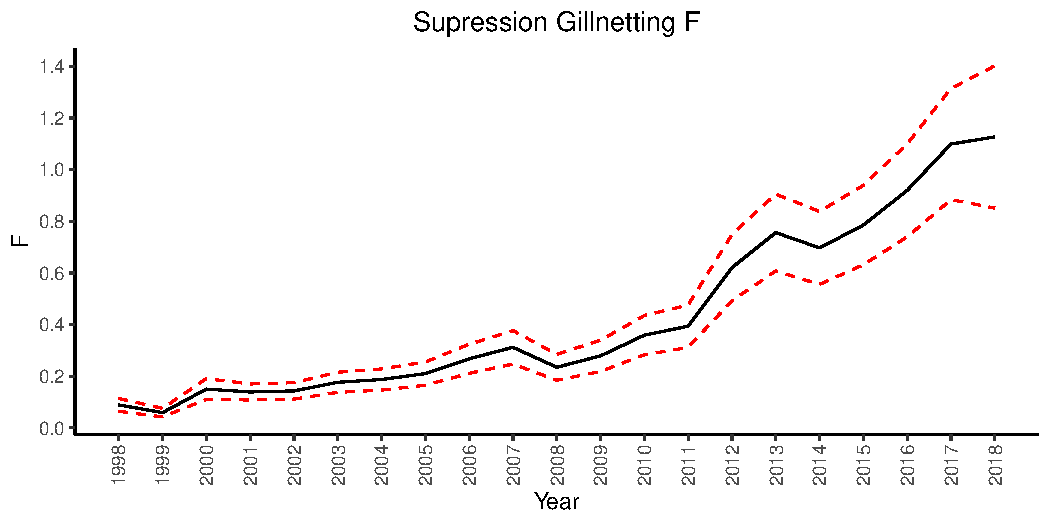
\includegraphics{Yellowstone-import-code_files/figure-latex/unnamed-chunk-2-1.pdf}

Figure 2. Estimates of fully selected instantaneous fishing mortality
(F) for suppression gillnetting for Yellowstone Lake lake trout from
\textbf{\texttt{1998}} through \textbf{\texttt{2018}} using a
statistical catch-at-age model. Dashed lines delineate 95\% confidence
intervals. \newline \newline \newline

\hypertarget{fig3}{%
\subsubsection{}\label{fig3}}

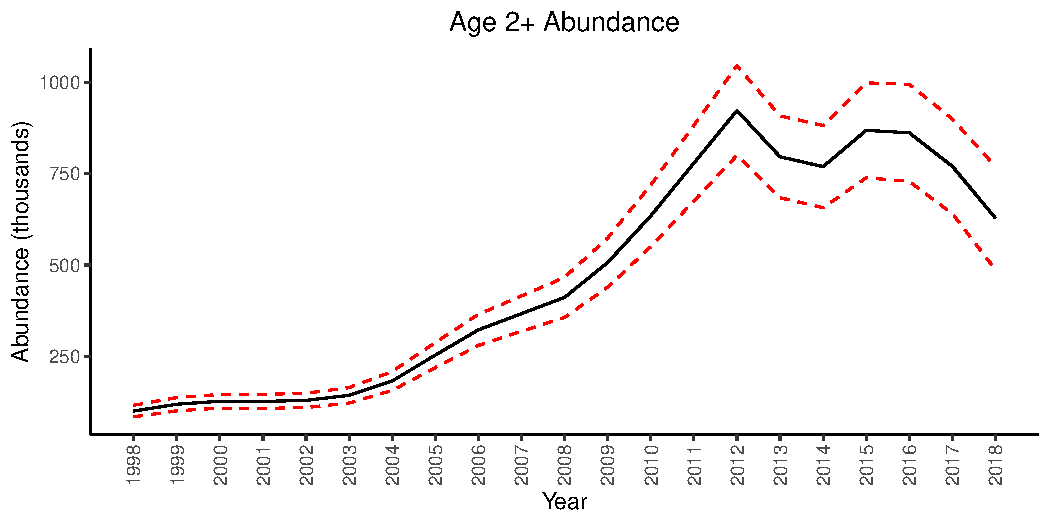
\includegraphics{Yellowstone-import-code_files/figure-latex/unnamed-chunk-3-1.pdf}

Figure 3. Abundance estimates for age-2 and older lake trout at the
start of the year for \textbf{\texttt{1998}} to \textbf{\texttt{2018}}
using a statistical catch-at-age model. Dashed lines delineate 95\%
confidence intervals. \pagebreak

\hypertarget{fig4}{%
\subsubsection{}\label{fig4}}

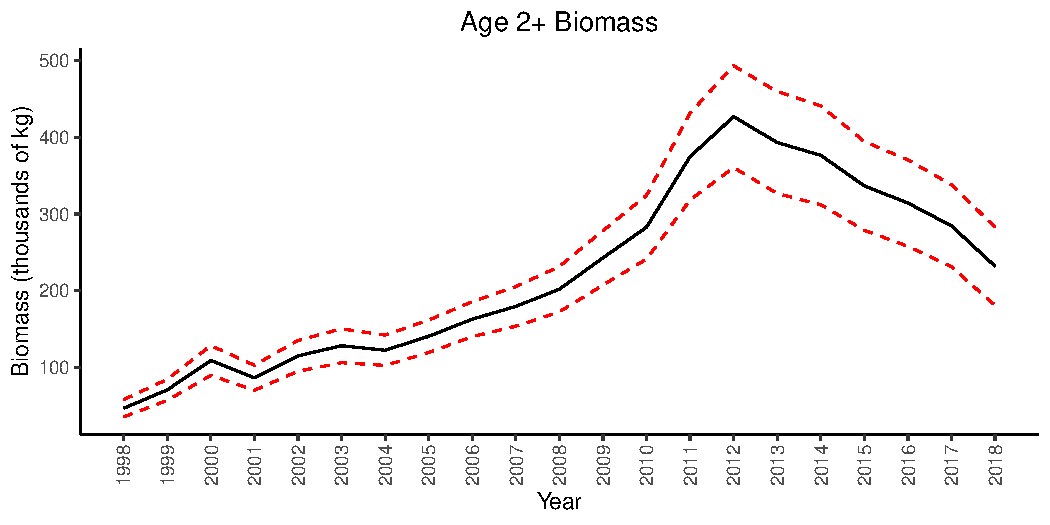
\includegraphics{Yellowstone-import-code_files/figure-latex/unnamed-chunk-4-1.pdf}

Figure 4. Biomass estimates for age-2 and greater lake trout from
\textbf{\texttt{1998}} through \textbf{\texttt{2018}} using a
statistical catch-at-age model. Dashed lines delineate 95\% confidence
intervals. \newline \newline \newline 

\hypertarget{fig5}{%
\subsubsection{}\label{fig5}}

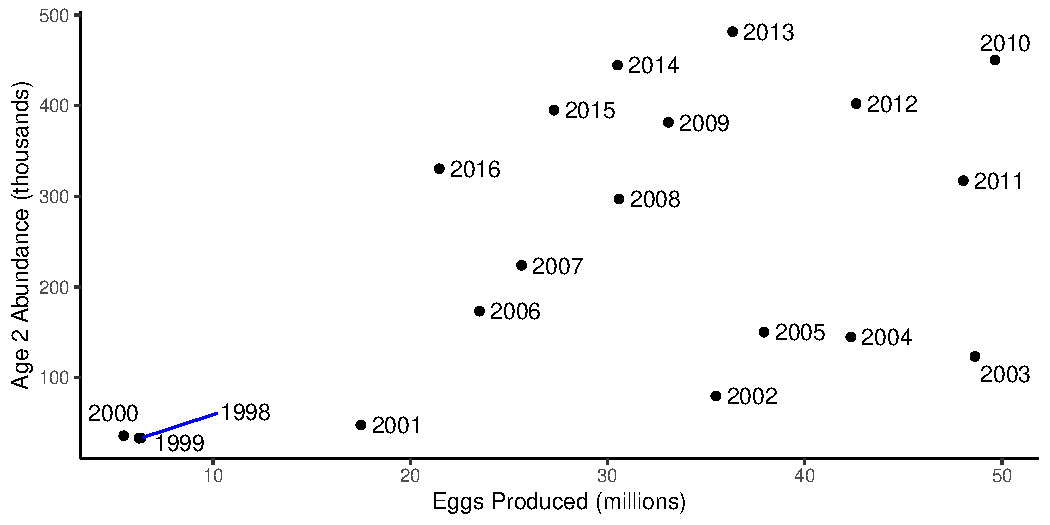
\includegraphics{Yellowstone-import-code_files/figure-latex/unnamed-chunk-5-1.pdf}

Figure 5. Age-2 lake trout abundance in relation to egg abundance,
lagged by 2 years. Labels indicate year class. The 1998, 1999, and 2000
year classes overlay one another in the bottom left corner of the
graph.\\
\pagebreak

\hypertarget{fig6}{%
\subsubsection{}\label{fig6}}

\begin{verbatim}
## Warning: ggrepel: 8 unlabeled data points (too many overlaps). Consider
## increasing max.overlaps
\end{verbatim}

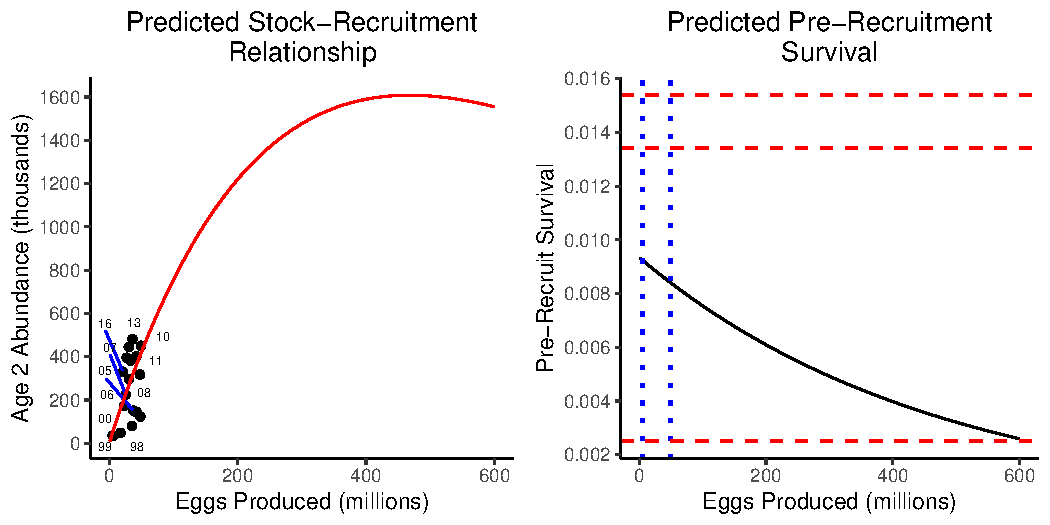
\includegraphics{Yellowstone-import-code_files/figure-latex/unnamed-chunk-6-1.pdf}

Figure 6. Predicted (black lines) Ricker stock-recruitment relationship
(left panel) and pre-recruit survival rates (right panel) using age-2
lake trout abundance as recruits and egg abundance as spawning stock
biomass for the \textbf{\texttt{1998}} to \textbf{\texttt{2016}} year
class. The points on the stock-recruitment graph are the observed
values. The red horizontal line on the pre-recruit survival graph
demarks early-life survival of lake trout from the scientific
literature.

\end{document}
